\documentclass{article}
\usepackage[utf8]{inputenc}
\usepackage{graphicx}

\title{Our first open source contribution.}
\author{Efthymia Kostaki \\
	 \texttt{ t8170055@aueb.gr}
	 \and
	 Stergios Sozos \\
 	 \texttt{t8170129@aueb.gr}
}
\date{May 2020}

\begin{document}
\maketitle

\begin{abstract}
Here will be a short paragraph about the contribution.
\end{abstract}

\section*{Introduction}
Blah blah blah
We worked together, but each one was assgined to a specific issue, and he undertook all the work on this issue, regarding branching, writing, communicating, opening PR and solving changes required. However, as stated before, we worked together for all issues, via teamviwer. Even though all the previous actions, were performed by one member, we were constantly ...klp

\section{Project Selection Process}
We utilized all the resources for finding an Open Source Project and we found more useful for us the site CodeTriange where we could explore different projects according to their programming language.
We organized the projects according to the frequency of update, the variety of contribution from different nationalities, gender etc. and how often where pull requests accepted, and issues generated. We focused mainly in JAVA and Python. 
We chose 3 of these OSS projects to install and build and also discussed with Mr Gkortzis our choices and their implementation. Due to operation system requirements (Windows) we disregarded one of them, Pretix, and focused on the other 2. We successfully built Mentorship Backend and that’s the project we worked on. It can be found here: https://github.com/anitab-org/mentorship-backend
Why we chose Mentorship Backend
\begin{itemize}
  \item Python language 
  \item Another entry in the list
  \item Use of Google Python Style Guide, contributing guidelines and general guidelines
  \item Communication on a daily basis on zulip chat
  \item Focus on issues for First Timers
  \item Interested in trying to contribute in the project also on the Android development part
\end{itemize}

\section{Initial Communication with the community}
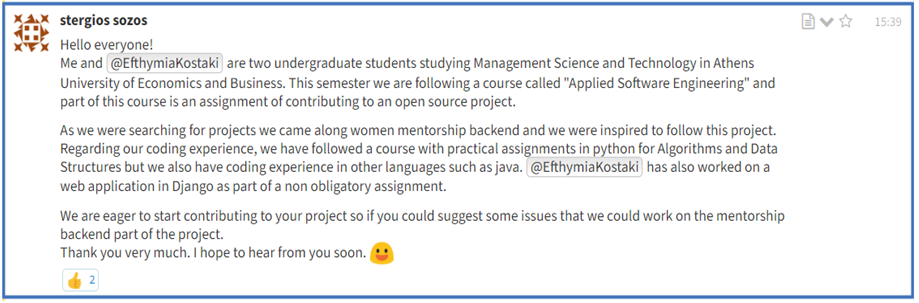
\includegraphics{FirstCommunication.png}

\section{Our contribution}
A section testing 

\subsection{Issue 1 - Create Quality Assurance table for Update Task API \#473}
Pull Request - Stergios

\subsubsection{Issue}
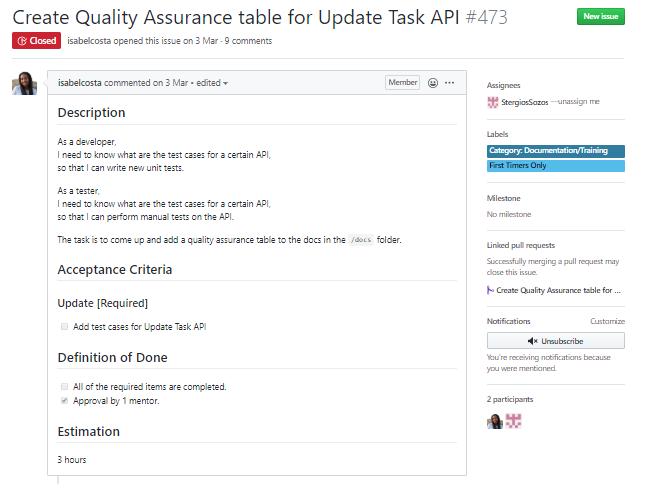
\includegraphics{issue473}

\subsubsection{Communication with the team}
A section

\subsubsection{More subsections}
A section

\subsection{Issue 2 -Fix description messages on Mentorship Relation \#554}
Pull Request - Stergios

\subsubsection{Issue}
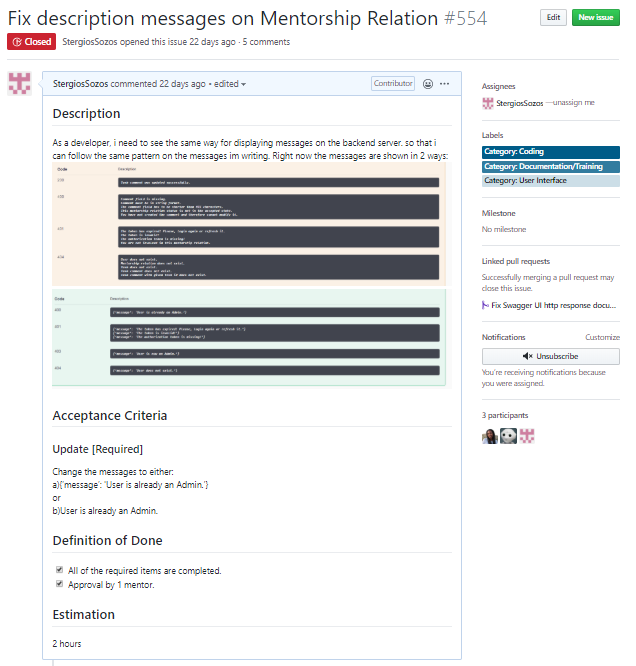
\includegraphics{issue554}

\subsubsection{Communication with the team}
A section

\subsubsection{Pull Request}
A section 

\subsubsection{Files changed}
ti alakse

\subsection{Issue 3 - "Complete task" not including all the necessary information when request id is not in accepted mode \#537}
Pull Request - Stergios

\subsubsection{Issue}
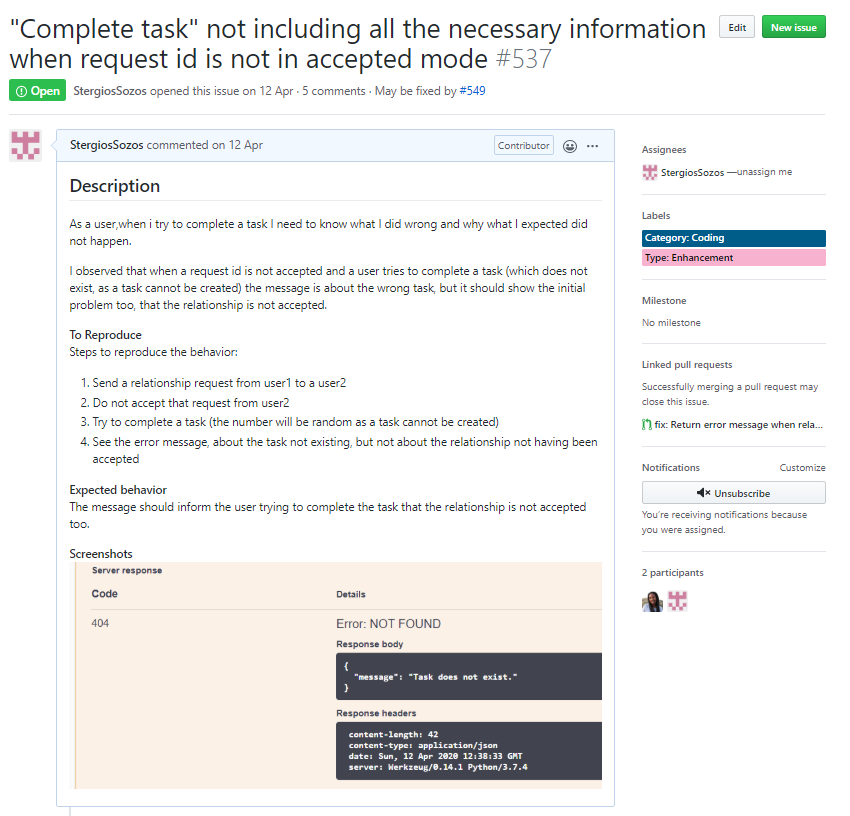
\includegraphics{issue537}

\subsubsection{Communication with the team}
A section

\subsubsection{More subsections}
A section

\subsection{Issue 4 - Title of issue to be added}
Pull Request - Efi


\subsubsection{Issue}
A section

\subsubsection{Communication with the team}
A section

\subsubsection{More subsections}
A section

\subsection{Issue 5 - Title of issue to be added}
Pull Request - Efi

\subsubsection{Issue}
A section

\subsubsection{Communication with the team}
A section

\subsubsection{More subsections}
A section

\subsection{Issue 6 - Title of issue to be added}
Pull Request - Efi

\subsubsection{Issue}
A section

\subsubsection{Communication with the team}
A section

\subsubsection{More subsections}
A section
\subsection{Issue 7 - Title of issue to be added}
Pull Request - Efi

\subsubsection{Issue}
A section

\subsubsection{Communication with the team}
A section

\subsubsection{More subsections}
A section

\end{document}